\newpage
\section{Example: Minesweeper}
In this section, we will develop a simple implementation of the well-known {\em Minesweeper} game.  Typically the minesweeper game is played through a graphical user interface, as illustrated by the following:
\begin{center}
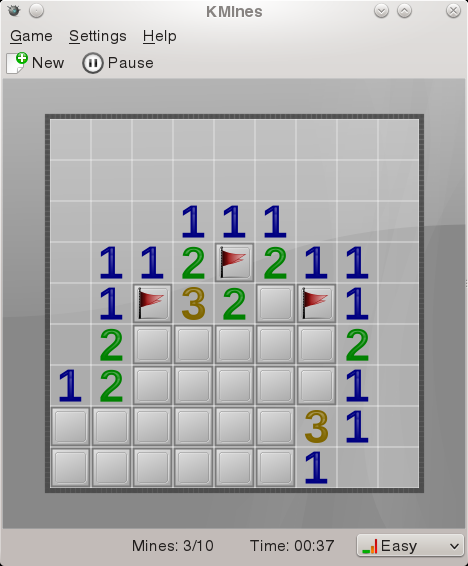
\includegraphics[width=0.4\textwidth]{../images/kmines.png}
\end{center}
Here, we can see the main aspects of the game.  The {\em game board} is a two-dimensional grid of {\em squares}.  Each square holds {\em nothing} or a {\em bomb} and is in one of the three states: {\em hidden}, {\em exposed} or {\em flagged} (with a flag).  An exposed square shows either the total number of bombs in the nine adjacent squares, referred to as its {\em rank}.  If an exposed square contains a bomb, then the game is over and the player has lost.  Flagged squares are protected and cannot be exposed unless they are {\em unflagged}.  The intuition here, is that the player marks those squares believed to contain a bomb.  

Let's analyse the above board.  In the following diagram of the above minesweeper game, gray squares represent hidden squares in the game.  For our benefit here, we've split them into two categories: those which contain a bomb (dark gray); and, those which don't: 

\begin{center}
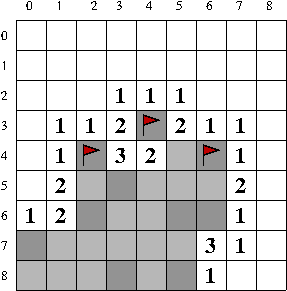
\includegraphics[width=0.4\textwidth]{../images/kmines_analysis.png}
\end{center}

In our discussion, we'll use $(x,y)$ to indicate a position on the board where $x$ gives the horizontal component, and $y$ the vertical component.  So, for example, the squares $(2,4)$, $(4,3)$ and $(6,4)$ are all marked with a flag.  Indeed, we can see that the above player has correctly flagged the three bombs in these squares, and that there are seven remaining to be identified and flagged.  Of course, unlike us, the player cannot see exactly where the bombs are.  However, he/she can easily determine that the square $(2,6)$ must contain a bomb.  This is because the exposed square at $(1,4)$ has a rank of $1$, and a bomb is flagged at $(2,4)$.  Therefore, there can be no bomb in square $(2,5)$ as this mean the rank of square $(1,4)$ was incorrect.  Finally, the rank of the square at $(1,5)$ is $2$ with only three unexposed squares, of which one is known already to contain a bomb and the other is known {\em not} to contain a bomb.  Therefore, the $(2,6)$ must contain a bomb.

The player plays the game by repeatedly selecting a square to expose.  When all squares are exposed, except for those containing bombs, the game is over and the player wins.  However, if a square holding a bomb is exposed, then the game is over immediately and the player loses.  A {\em blank} square is one with no adjacent bombs.  When a blank square is exposed, every adjacent blank square is recursively exposed.

